\documentclass{article}

\usepackage{fancyhdr}
\usepackage{extramarks}
\usepackage{amsmath}
\usepackage{amsthm}
\usepackage{amsfonts}
\usepackage{tikz}
\usepackage[plain]{algorithm}
\usepackage{algpseudocode}
\usepackage{physics}

\usetikzlibrary{automata,positioning}

%
% Basic Document Settings
%

\topmargin=-0.45in
\evensidemargin=0in
\oddsidemargin=0in
\textwidth=6.5in
\textheight=9.0in
\headsep=0.25in

\linespread{1.1}

\pagestyle{fancy}
\lhead{\hmwkAuthorName}
\chead{\hmwkClass\ (\hmwkClassInstructor\ \hmwkClassTime): \hmwkTitle}
\rhead{\firstxmark}
\lfoot{\lastxmark}
\cfoot{\thepage}

\renewcommand\headrulewidth{0.4pt}
\renewcommand\footrulewidth{0.4pt}

\setlength\parindent{0pt}

%
% Create Problem Sections
%

\newcommand{\enterProblemHeader}[1]{
    \nobreak\extramarks{}{Problem \arabic{#1} continued on next page\ldots}\nobreak{}
    \nobreak\extramarks{Problem \arabic{#1} (continued)}{Problem \arabic{#1} continued on next page\ldots}\nobreak{}
}

\newcommand{\exitProblemHeader}[1]{
    \nobreak\extramarks{Problem \arabic{#1} (continued)}{Problem \arabic{#1} continued on next page\ldots}\nobreak{}
    \stepcounter{#1}
    \nobreak\extramarks{Problem \arabic{#1}}{}\nobreak{}
}

\setcounter{secnumdepth}{0}
\newcounter{partCounter}
\newcounter{homeworkProblemCounter}
\setcounter{homeworkProblemCounter}{1}
\nobreak\extramarks{Problem \arabic{homeworkProblemCounter}}{}\nobreak{}

%
% Homework Problem Environment
%
% This environment takes an optional argument. When given, it will adjust the
% problem counter. This is useful for when the problems given for your
% assignment aren't sequential. See the last 3 problems of this template for an
% example.
%
\newenvironment{homeworkProblem}[1][-1]{
    \ifnum#1>0
        \setcounter{homeworkProblemCounter}{#1}
    \fi
    \section{Problem \arabic{homeworkProblemCounter}}
    \setcounter{partCounter}{1}
    \enterProblemHeader{homeworkProblemCounter}
}{
    \exitProblemHeader{homeworkProblemCounter}
}

%
% Homework Details
%   - Title
%   - Due date
%   - Class
%   - Section/Time
%   - Instructor
%   - Author
%

\newcommand{\hmwkTitle}{Assignment 4}
\newcommand{\hmwkDueDate}{February 26, 2024}
\newcommand{\hmwkClass}{COMP 4200}
\newcommand{\hmwkClassTime}{001}
\newcommand{\hmwkClassInstructor}{Professor Kwon}
\newcommand{\hmwkAuthorName}{\textbf{Matthew Rogers}}

%
% Title Page
%

\title{
    \vspace{2in}
    \textmd{\textbf{\hmwkClass:\ \hmwkTitle}}\\
    \normalsize\vspace{0.1in}\small{Due\ on\ \hmwkDueDate}\\
    \vspace{0.1in}\large{\textit{\hmwkClassInstructor\ \hmwkClassTime}}
    \vspace{3in}
}

\author{\hmwkAuthorName}
\date{}

\renewcommand{\part}[1]{\textbf{\large Part \Alph{partCounter}}\stepcounter{partCounter}\\}

%
% Various Helper Commands
%

% Useful for algorithms
\newcommand{\alg}[1]{\textsc{\bfseries \footnotesize #1}}

% For derivatives
\newcommand{\deriv}[1]{\frac{\mathrm{d}}{\mathrm{d}x} (#1)}

% For partial derivatives
\newcommand{\pderiv}[2]{\frac{\partial}{\partial #1} (#2)}

% Integral dx
\newcommand{\dx}{\mathrm{d}x}

% Alias for the Solution section header
\newcommand{\solution}{\textbf{\large Solution}}

% Probability commands: Expectation, Variance, Covariance, Bias
\newcommand{\E}{\mathrm{E}}
\newcommand{\Var}{\mathrm{Var}}
\newcommand{\Cov}{\mathrm{Cov}}
\newcommand{\Bias}{\mathrm{Bias}}

\begin{document}

\maketitle

\pagebreak

\begin{homeworkProblem}
    Convert the following regular expressions into equivalent NFAs.

    \begin{enumerate}
        \item $a^\ast(b\cup c)^\ast c$
        \item $({(b\cup a)}^\ast \cup (c \cup a))^\ast(cb)^\ast$ \\
    \end{enumerate}
    \textbf{Solution}\\
    \textbf{Part One}
        \begin{figure}[h]
        \centering
        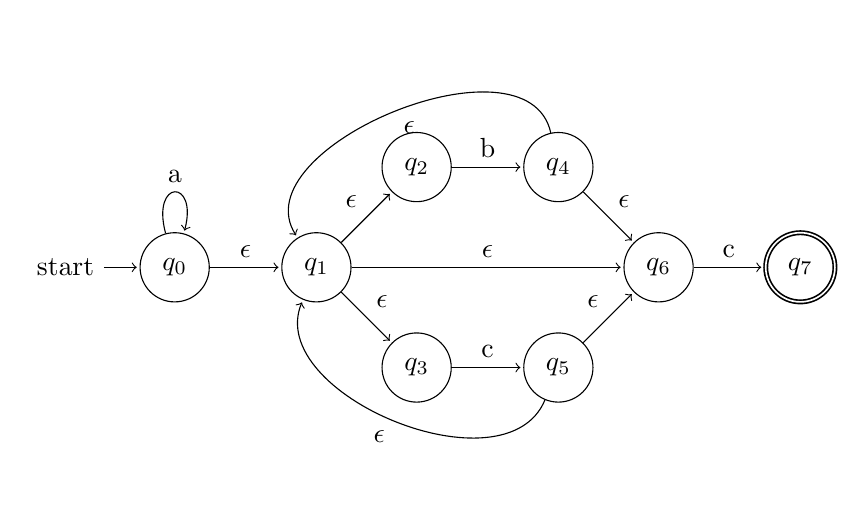
\begin{tikzpicture}[shorten >=1pt,node distance=1.8cm,on grid,auto]
            \node[state, initial] (q_0) {$q_0$};
            \node[state] (q_1) [right=of q_0] {$q_1$};
            \node[state] (q_2) [above right=of q_1] {$q_2$};
            \node[state] (q_3) [below right=of q_1] {$q_3$};
            \node[state] (q_4) [right=of q_2] {$q_4$};
            \node[state] (q_5) [right=of q_3] {$q_5$};
            \node[state] (q_6) [above right=of q_5] {$q_6$};
            \node[state, accepting, semithick] (q_7) [right=of q_6] {$q_{7}$};
            \path[->]
                (q_0)
                    edge node {$\epsilon$} (q_1)
                    edge [loop above] node {a} (q_0)
                (q_1)
                    edge node {$\epsilon$} (q_2)
                    edge node {$\epsilon$} (q_3)
                    edge node {$\epsilon$} (q_6)
                (q_2)
                    edge node {b} (q_4)
                (q_3)
                    edge node {c} (q_5)
                (q_4)
                    edge [bend right=100] node {$\epsilon$} (q_1)
                    edge node {$\epsilon$} (q_6)
                (q_5)
                    edge [bend left=90] node {$\epsilon$} (q_1)
                    edge node {$\epsilon$} (q_6)
                (q_6)
                    edge node {c} (q_7);
        \end{tikzpicture}
    \end{figure}

    \textbf{Part Two}
    \begin{figure}[h]
        \centering
        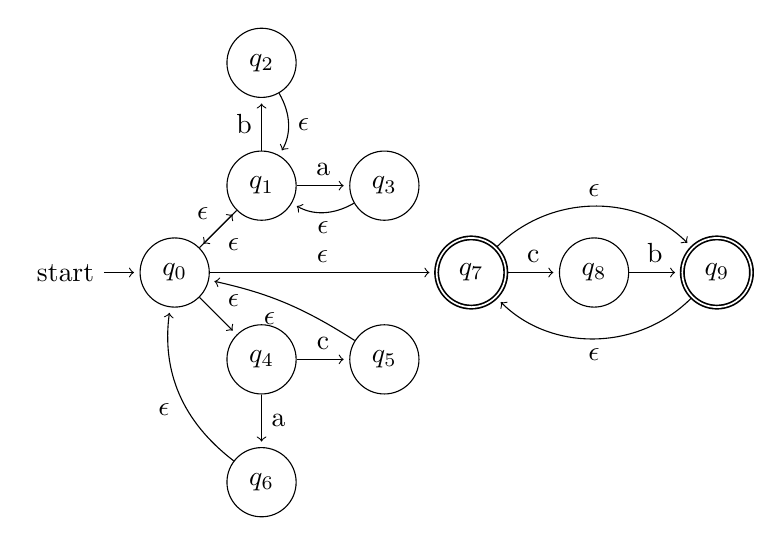
\begin{tikzpicture}[shorten >=2pt,node distance=1.56cm,on grid,auto]
            \node[state, initial] (q_0)   {$q_0$};
            \node[state] (q_1) [above right=of q_0] {$q_1$};
            \node[state] (q_2) [above=of q_1] {$q_2$};
            \node[state] (q_3) [right=of q_1] {$q_3$};
            \node[state] (q_4) [below right=of q_0] {$q_4$};
            \node[state] (q_5) [right=of q_4] {$q_5$};
            \node[state] (q_6) [below=of q_4] {$q_6$};
            \node[state, accepting, semithick] (q_7) [below right=of q_3] {$q_7$};
            \node[state] (q_8) [right=of q_7] {$q_8$};
            \node[state, accepting, semithick] (q_9) [right=of q_8] {$q_9$};
            \path[->]
                (q_0)
                    edge node {$\epsilon$} (q_1)
                    edge node {$\epsilon$} (q_4)
                    edge node {$\epsilon$} (q_7)
                (q_1)
                    edge node {b} (q_2)
                    edge node {a} (q_3)
                    edge node {$\epsilon$} (q_0)
                (q_2)
                    edge [bend left] node {$\epsilon$} (q_1)
                (q_3)
                    edge [bend left] node {$\epsilon$} (q_1)
                (q_4)
                    edge node {c} (q_5)
                    edge node {a} (q_6)
                (q_5)
                    edge [bend right=10] node {$\epsilon$} (q_0)
                (q_6)
                    edge [bend left] node {$\epsilon$} (q_0)
                (q_7)
                    edge node {c} (q_8)
                    edge [bend left=45] node {$\epsilon$} (q_9)
                (q_8)
                    edge node {b} (q_9)
                (q_9)
                    edge [bend left=45] node {$\epsilon$} (q_7)
                ;
        \end{tikzpicture}
    \end{figure}

\end{homeworkProblem}
\newpage
\begin{homeworkProblem}
    Convert the 2 NFA's to equivalent regular expressions. \\
    \textbf{Solution} \\

    \textbf{Part One}\\
    1. Convert NFA to GNFA \\
    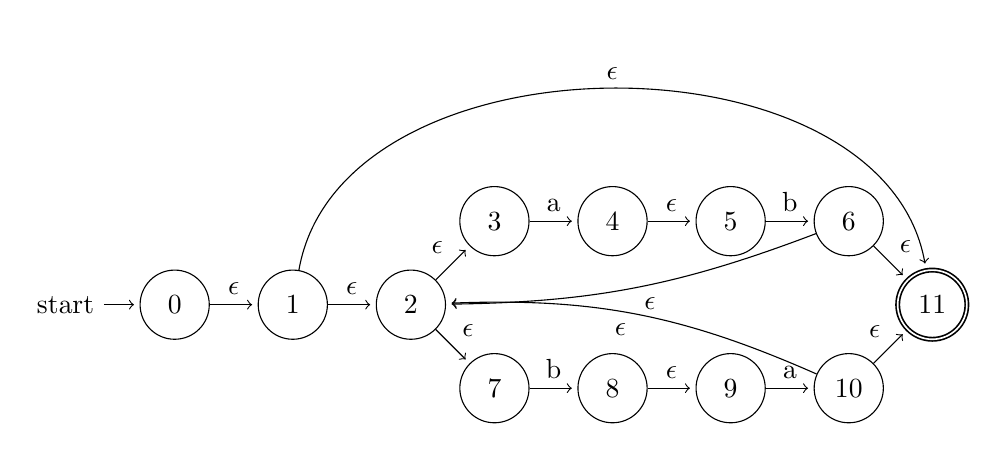
\begin{tikzpicture}[shorten >=2pt,node distance=1.5cm,on grid,auto]
        \node[state, initial] (q_0) {$0$};
        \node[state] (q_1) [right=of q_0]  {$1$};
        \node[state] (q_2) [right=of q_1] {$2$};
        \node[state] (q_3) [above right =of q_2] {$3$};
        \node[state] (q_4) [right=of q_3] {$4$};
        \node[state] (q_5) [right=of q_4] {$5$};
        \node[state] (q_6) [right=of q_5] {$6$};
        \node[state] (q_7) [below right=of q_2] {$7$};
        \node[state] (q_8) [right=of q_7] {$8$};
        \node[state] (q_9) [right=of q_8] {$9$};
        \node[state] (q_10) [right=of q_9] {$10$};
        \node[state, accepting, semithick] (q_11) [above right=of q_10] {$11$};
        \path[->]
            (q_0)
                edge node {$\epsilon$} (q_1)
            (q_1)
                edge node {$\epsilon$} (q_2)
                edge [bend left=80] node {$\epsilon$} (q_11)
            (q_2)
                edge node {$\epsilon$} (q_3)
                edge node {$\epsilon$} (q_7)
            (q_3)
                edge node {a} (q_4)
            (q_4)
                edge node {$\epsilon$} (q_5)
            (q_5)
                edge node {b} (q_6)
            (q_6)
                edge [bend left=10] node {$\epsilon$} (q_2)
                edge node {$\epsilon$} (q_11)
            (q_7)
                edge node {b} (q_8)
            (q_8)
                edge node {$\epsilon$} (q_9)
            (q_9)
                edge node {a} (q_10)
            (q_10)
                edge [bend right=13] node {$\epsilon$} (q_2)
                edge node {$\epsilon$} (q_11);
    \end{tikzpicture} \\

    2. Fix 3,4,5 and 7,8,9. These are trivial and can be summarized by $2\xrightarrow{ab} 6$ and $2\xrightarrow{ba} 10$ \\
    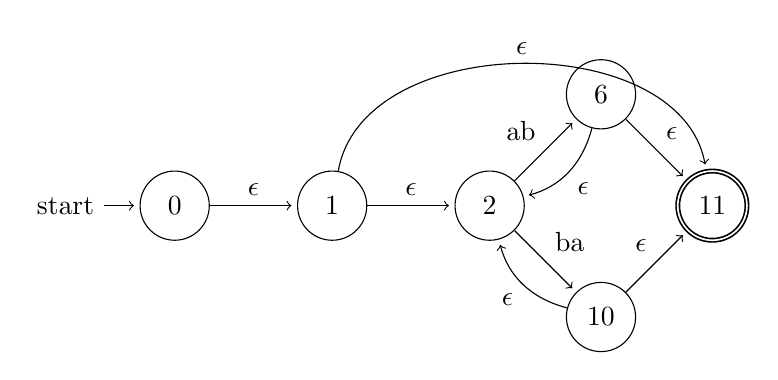
\begin{tikzpicture}[shorten >=2pt,node distance=2cm,on grid,auto]
        \node[state, initial] (q_0) {$0$};
        \node[state] (q_1) [right=of q_0] {$1$};
        \node[state] (q_2) [right=of q_1] {$2$};
        \node[state] (q_6) [above right=of q_2] {$6$};
        \node[state] (q_10) [below right=of q_2] {$10$};
        \node[state, accepting, semithick] (q_11) [above right=of q_10] {$11$};
        \path[->]
            (q_0)
                edge node {$\epsilon$} (q_1)
            (q_1)
                edge node {$\epsilon$} (q_2)
                edge [bend left=80] node {$\epsilon$} (q_11)
            (q_2)
                edge node {ab} (q_6)
                edge node {ba} (q_10)
            (q_6)
                edge [bend left] node {$\epsilon$} (q_2)
                edge node {$\epsilon$} (q_11)
            (q_10)
                edge [bend left] node {$\epsilon$} (q_2)
                edge node {$\epsilon$} (q_11);

    \end{tikzpicture} \\

    3. Fix 6,10. 6 yields $2\xrightarrow{ab} 2$ and $2\xrightarrow{ab} 11$. 10 yields $2\xrightarrow{ba} 2$ and $2\xrightarrow{ba} 11$. Finally, $2\xrightarrow{ab \cup ba} 2$ and $2\xrightarrow{ab \cup ba} 11$\\
    \begin{tikzpicture}[shorten >=2pt,node distance=2cm,on grid,auto]
        \node[state, initial] (q_0) {$0$};
        \node[state] [right=of q_0]   {$1$};
        \node[state] (q_2) [right=of q_1] {$2$};
        \node[state, accepting, semithick] (q_11) [right=of q_2] {$11$};
        \path[->]
            (q_0)
                edge node {$\epsilon$} (q_1)
            (q_1)
                edge node {$\epsilon$} (q_2)
                edge [bend right=45] node {$\epsilon$} (q_11)
            (q_2)
                edge [loop above] node {$ab\cup ba$} (q_2)
                edge node {$ab\cup ba$} (q_11);
    \end{tikzpicture} \\

    4. Fix 2. $1\xrightarrow{((ab\cup ba)^*ab\cup ba)\cup\epsilon} 11$\\
    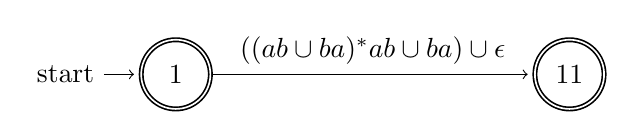
\begin{tikzpicture}[shorten >=2pt,node distance=5cm,on grid,auto]
        \node[state, initial, accepting, semithick] (q_1)   {$1$};
        \node[state, accepting, semithick] (q_11) [right=of q_1] {$11$};
        \path[->]
            (q_1)
                edge node {$((ab\cup ba)^*ab\cup ba)\cup\epsilon$} (q_11);
    \end{tikzpicture} \\

    RE: $((ab\cup ba)^*ab\cup ba)\cup\epsilon$\\

    \newpage
    \textbf{Part Two} \\
    1. Convert NFA to GNFA\\
    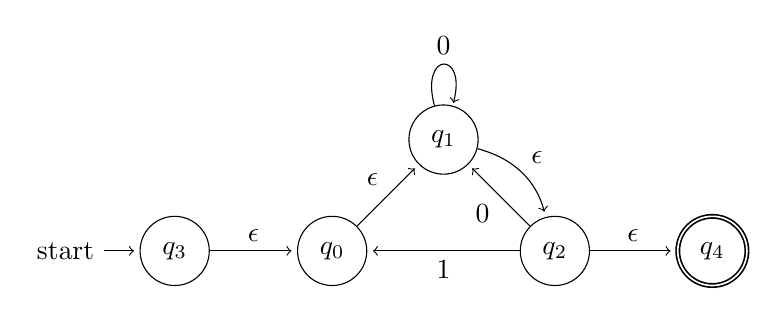
\begin{tikzpicture}[shorten >=2pt,node distance=2cm,on grid,auto]
        \node[state] (q_0)   {$q_0$};
        \node[state] (q_1) [above right=of q_0] {$q_1$};
        \node[state] (q_2) [below right=of q_1] {$q_2$};
        \node[state, initial] (q_3) [left=of q_0] {$q_3$};
        \node[state, accepting, semithick] (q_4) [right=of q_2] {$q_4$};
        \path[->]
            (q_3)
                edge node {$\epsilon$} (q_0)
            (q_0)
                edge node {$\epsilon$} (q_1)
            (q_1)
                edge [loop above] node {0} (q_1)
                edge [bend left] node {$\epsilon$} (q_2)
            (q_2)
                edge node {0} (q_1)
                edge node {1} (q_0)
                edge node {$\epsilon$} (q_4);
    \end{tikzpicture} \\

    2. Fix $q_0$: $q_3\xrightarrow{\epsilon} q_1$, $q_2\xrightarrow{1} q_1$ \\
    \begin{tikzpicture}[shorten >=2pt,node distance=2cm,on grid,auto]
        \node[state] (q_1) {$q_1$};
        \node[state] (q_2) [right=of q_1] {$q_2$};
        \node[state, initial] (q_3) [left=of q_0] {$q_3$};
        \node[state, accepting, semithick] (q_4) [right=of q_2] {$q_4$};
        \path[->]
            (q_3)
                edge node {$\epsilon$} (q_1)
            (q_1)
                edge [loop above] node {0} (q_1)
                edge [bend left] node {$\epsilon$} (q_2)
            (q_2)
                edge node {$0 \cup 1$} (q_1)
                edge node {$\epsilon$} (q_4);
    \end{tikzpicture} \\

    3. Fix $q_2$: $q_1\xrightarrow{0 \cup 1} q_1$, $q_1\xrightarrow{\epsilon} q_4$ \\
    \begin{tikzpicture}[shorten >=2pt,node distance=2cm,on grid,auto]
        \node[state] (q_1) {$q_1$};
        \node[state, initial] (q_3) [left=of q_0] {$q_3$};
        \node[state, accepting, semithick] (q_4) [right=of q_1] {$q_4$};
        \path[->]
            (q_3)
                edge node {$\epsilon$} (q_1)
            (q_1)
                edge [loop above] node {$0 \cup 1$} (q_1)
                edge node {$\epsilon$} (q_4);
    \end{tikzpicture} \\

    RE: $(0 \cup 1)^*$\\ 
\end{homeworkProblem}

\begin{homeworkProblem}
    Prove the regularity of the languages. If regular, construct a DFA, NFA, or RE.
    \begin{enumerate}
        \item $X=\{0^m1^n\mid m>n\geq0\}$
        \item $Y=\{0^n\mid n \text{ is a prime}\}$
    \end{enumerate}
    \textbf{Part One}\\

    Assume $X$ is regular. \\
    Let $s=0^{P+1}1^P$. $P+1>P$. So for all $P\geq0$, $s\in X$.\\
    $\abs{s}=2P+1$, which is $\geq P$. \\
    Let $xy=0^P$. So $\abs{xy}=P$. And we can represent s as $xy01^P$. \\
    $y$ will be some amount of 0's. For any $y=0^n$ where $n>2$, when you pump down, the number of leading zeros will be less than P. Then $m\not>n$. Then s is not in X, and we arrive at a contradiction. Therefore, X is non-regular. \\

    \textbf{Part Two}\\

    Assume $Y$ is regular. \\
    Let $s=0^P$, where $P$ is a prime number.\\
    $\abs{s}=P$, which is $\geq P$. \\
    Let $xy=0^P$. So $\abs{xy}=P$. \\
    $y$ will be some amount of 0's. After 2, there are no even prime numbers. Therefore for approximately half of all y-pumps, $\abs{xy}$ is not a prime number. $Y$ is not pumpable and we arrive at a contradiction. Therefore, Y is non-regular.



\end{homeworkProblem}

\end{document}